\documentclass[Contributo.tex]{subfiles}

\begin{document}
\subsection{Estensione della sintassi del linguaggio}
La sintassi del linguaggio mostrata in 2.2 viene estesa tramite queste 4 espressioni e mostrata in figura \ref{newrules}:
\begin{itemize}
	\item $\displaystyle \mathsf{process\_flag}(\mathsf{trap\_exit},Boolean)\xrightarrow{return}OldBool$: Se \textit{Boolean}=$\mathsf{true}$, i segnali di uscita che arrivano al processo chiamante vengono convertiti in messaggi \textit{\{'EXIT', From, Reason\}}, che possono essere ricevuti come messaggi ordinari. 
	Se \textit{Boolean}=$\mathsf{false}$, il processo chiamante \textit{termina} se riceve un segnale di uscita diverso da \textit{Reason}=$\mathsf{normal}$, \textbf{che a sua volta viene ripropagato a tutti i processi collegati con esso e cosi vià}.
	La chiamata a $\mathsf{process\_flag}$ ritorna il valore del vecchio flag(\textit{OldBool}).
	\item $\displaystyle \mathsf{spawn\_link}(expr, [expr_{1},...,expr_{n}])\xrightarrow{return}SpawnedPid$: funziona esattamente per la $\mathsf{spawn}$, con l'aggiunta che il processo spawnato si linka \textit{atomicamente} con \textit{SpawnedPid}.
	\item $\displaystyle \mathsf{exit}(Reason)\xrightarrow{no\_return}$: il processo chiamante termina con motivo di uscita Reason.
	Se \textit{Reason}=$\mathsf{normal}$, viene intesa come \textit{normale} terminazione del codice, altrimenti segnala una terminazione \textit{anomala} con motivo \textit{Reason}.
	\item $\displaystyle \mathsf{error}(Reason)\xrightarrow{no\_return}$: il processo chiamante termina in modo \textit{anomalo} la sua esecuzione con motivo \textit{Reason}.
	A differenza di $\mathsf{exit}$, $\mathsf{error}$ segnala \textbf{sempre} un errore durante l'esecuzione.
	Errori a run-time, tipo divisioni per 0 ecc., equivalgono ad una chiamata a $\mathsf{error}$, con la relativa \textit{Reason}.
\end{itemize}
\begin{figure}[!ht]
  $\displaystyle
  \begin{array}{rcl@{~~~~~~}l}
    \mathit{module} & ::= & \mathsf{module} ~ Atom = %%[fname_1,\ldots,fname_n] =
    \mathit{fun}_1,\ldots,\mathit{fun}_n\\
    {\mathit{fun}} & ::= & \mathit{fname} = \mathsf{fun}~(X_1,\ldots,X_n) \to expr \\
    {\mathit{fname}} & ::= & Atom/Integer \\
    lit & ::= & Atom \mid Integer \mid Float \mid \nil \\
    expr & ::= & \mathit{Var} \mid lit \mid \mathit{fname} \mid [expr_1|expr_2]
                 \mid   \{expr_1,\ldots,expr_n\} \\
    & \mid & \mathsf{call}~expr~(expr_1,\ldots,expr_n) 
    \mid \mathsf{apply}~expr~(expr_1,\ldots,expr_n) \\
    & \mid &
    \mathsf{case}~expr~\mathsf{of}~clause_1;\ldots;clause_m~\mathsf{end}\\
    & \mid & \mathsf{let}~\mathit{Var}=expr_1~\mathsf{in}~expr_2 
    \mid \mathsf{receive}~clause_1;\ldots;clause_n~\mathsf{end}\\
    & \mid & \mathsf{spawn}(expr,[expr_1,\ldots,expr_n])  \mid \mathsf{spawn\_link}(expr,[expr_1,\ldots,expr_n])\\
    & \mid & expr_1 \:!\: expr_2 \mid \mathsf{self}() \mid \mathsf{process\_flag}(\mathsf{trap\_exit},Atom)\\
    & \mid & \mathsf{error}(lit) \mid \mathsf{exit}(lit)\\
     clause & ::= & pat ~\mathsf{when}~expr_1 \to expr_2
    \\
    pat & ::= & \mathit{Var} \mid lit \mid [pat_1|pat_2] \mid
    \{pat_1,\ldots,pat_n\} \\
  \end{array}
  $
\caption{Regole sintattiche del linguaggio esteso} 
\label{newrules}
\end{figure}
\subsection{Estensione delle strutture dati del linguaggio}
Il sistema S=$\displaystyle \Gamma;\Pi$ si estende in S=$\displaystyle \Gamma;\Psi;\Pi$, ove $\Psi$ denota la \textit{global signal box}, che è un \textit{insieme} di \textit{signal}, derivanti dalla terminazione di un \textit{processo}, e in attesa di essere consegnati.
Ciò in Cauder si traduce con l'aggiunta al tipo \textit{record sys} di un campo \textit{signals=[]} che corrisponde a $\Psi$.
Lo \textit{scheduler} viene modificato tramite l'estensione dell'opzione PRIO\_RANDOM, in cui viene data priorità anche ai \textit{segnali} assieme ai \textit{processi}.
\textit{Signal} è una tupla del tipo \textit{\{p',p,type,reason,time\}} dove:
	\begin{itemize}
		\item \textit{p'} denota il pid del processo a cui recapitare il segnale.
		\item \textit{p} denota il pid del processo che ha generato il segnale.
		\item \textit{type}=$\mathsf{error}$ oppure $\mathsf{normal}$ denota il tipo di segnale, ovvero un errore o una terminazione normale del codice.
		\item \textit{reason} denota, nel caso di errore, la ragione per cui l'errore si è verificato.
			  Nel caso di \textit{type}=$\mathsf{normal}$, \textit{reason} sarà uguale ad $\mathsf{undefined}$.
		\item \textit{time} analogo come per i messaggi.Da notare che, \textbf{in questa specifica estensione}, il campo \textit{time} non è necessario per la discriminazione dei segnali in sè, bensì, nel caso il \textit{flag} del processo ricevente fosse $\mathsf{true}$ e quindi quel segnale fosse convertito in messaggio, serve per discriminare quel particolare messaggio che verrà creato.
	\end{itemize}
In Cauder \textit{Signal} si traduce nel tipo \textit{record signal} composto da:
	\begin{itemize}
		\item \textit{dest} = \textit{p'} 
		\item \textit{from} = \textit{p}
		\item \textit{type} = \textit{type}
		\item \textit{reason} = \textit{reason}
		\item \textit{time} = \textit{time}
	\end{itemize}
La struttura di un processo P=$\displaystyle \langle p,\theta,e,h,lm \rangle$ si estende in P=$\displaystyle \langle p,\theta,e,h,lm,l,f \rangle$ dove:
	\begin{itemize}
		\item \textit{l} denota l'insieme dei \textit{pid} con cui il processo è linkato.
		\item \textit{f} denota il valore del \textit{process\_flag} del processo.
	\end{itemize}
In Cauder si traduce nell'aggiunta, al tipo \textit{record proc} di un campo \textit{flag=false} e \textit{links=[]}.\\
La figura sottostante mostra graficamente lo stato di Cauder esteso. Viene aggiunto \textit{GS} che corrisponde a $\Psi$ (\textit{signals}), mentre la struttura dati del processo viene estesa tramite l'aggiunta di \textit{PROC\_FLAG} che corrisponde a \textit{f} (\textit{flag}) ed \textit{LINKS} che corrisponde ad \textit{l} (\textit{links}).
\begin{figure}[H]
		\centerline{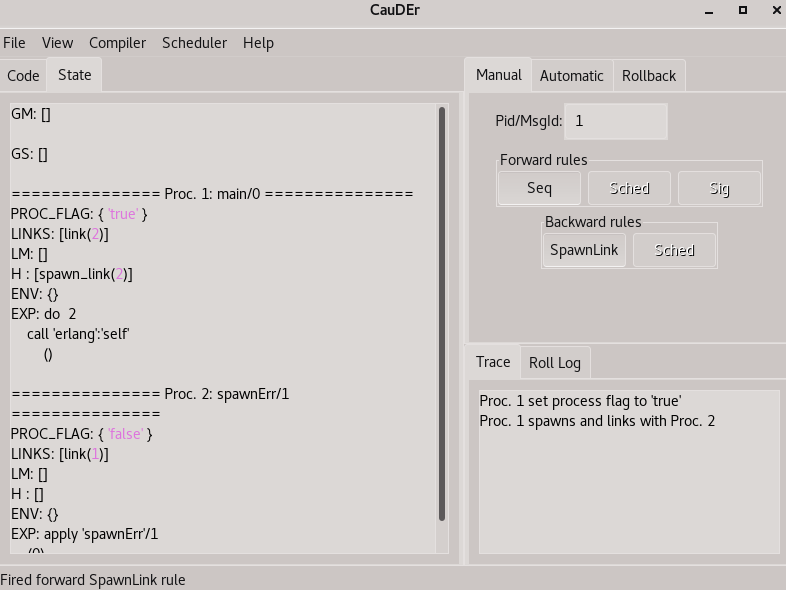
\includegraphics[scale=0.5]{./LavoroLuca/EstensioneCauder/Imgs/CauderStatoEsteso}}
		\caption{Stato di Cauder esteso.}
		\label{fig4}
	\end{figure}
\subsection{Estensione della semantica}
Ora che è stata introdotta la nuova sintassi, spiegando quali funzioni vengono aggiunte e quali effetti producono, assieme alle nuove features di sistema, andrò a definire, \textbf{come nel punto 3 della sezione 2.2}, la semantica reversibile estesa del nuovo linguaggio, lavorando su un processo generico P esteso \textit{che esegue la regola descritta}, ovvero $\displaystyle \langle p,\theta,e,h,lm,l,f \rangle$ e su un sistema generico S esteso, ovvero $\displaystyle \Gamma;\Psi;\Pi$.\\
\textbf{SEMANTICA IN AVANTI}:\\
	Alle varie regole che seguiranno, associerò la loro relativa rappresentazione grafica utilizzando il tool \textit{Graphic Viewer} integrato in Cauder. Qui sotto riporto alcune immagini di esempio in cui spiego a grandi linee come interpretare le visualizzazioni del \textit{Graphic Viewer}, con riferimento a \cite{et}.\\
	In relazione alla figura sottostante, i numeri rossi in alto, sopra le linee verticali colorate, indicano il pid di un processo. Le linee verticali possono assumere due colorazioni: \textit{verde} se il processo è presente nel sistema ed è attivo, \textit{rosso} se il processo è presente nel sistema ma non è attivo. Una freccia uscente da un pallino, indica un'azione eseguita da un processo verso un altro processo, con la relativa \textit{label} sopra di essa, indicante che tipo di azione viene eseguita. Se un'azione non coinvolge un secondo processo oppure si ha un invio di qualche informazione \underline{senza aver effettuato la relativa ricezione} (vedi \textit{send} qui sopra), allora verrà rappresentato solo da un pallino, composta dalla \textit{label e dalla relativa informazione}.
	\begin{figure}[H]
		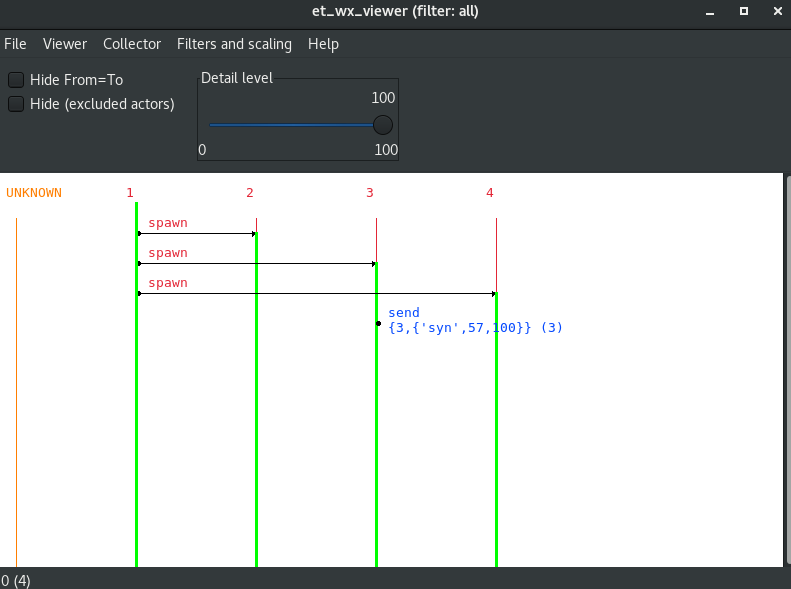
\includegraphics[scale=0.5]{./LavoroLuca/EstensioneCauder/Imgs/GraphicViewerSend}
		\caption{Esempio Graphic Viewer}
		\label{fig5}
	\end{figure}
	Invece, nella figura sottostante, vediamo la ricezione della send della figura precedente. Uso una freccia \textit{obliqua}, in modo da evidenziare l'asincronia nella comunicazione di Erlang.
	La label sopra la freccia riporta l'informazione scambiata.\\
	L'informazione è composta dal \textit{payload}, quindi il vero contenuto informativo e dal \textit{time}, che risulta \textbf{sempre} visibile, tra le parentesi tonde a fine label. Questo esempio riprende la send della figura precedente. Questo tipo di visualizzazione verrà usato anche per la propagazione e ricezione di segnali.
	\begin{figure}[H]
		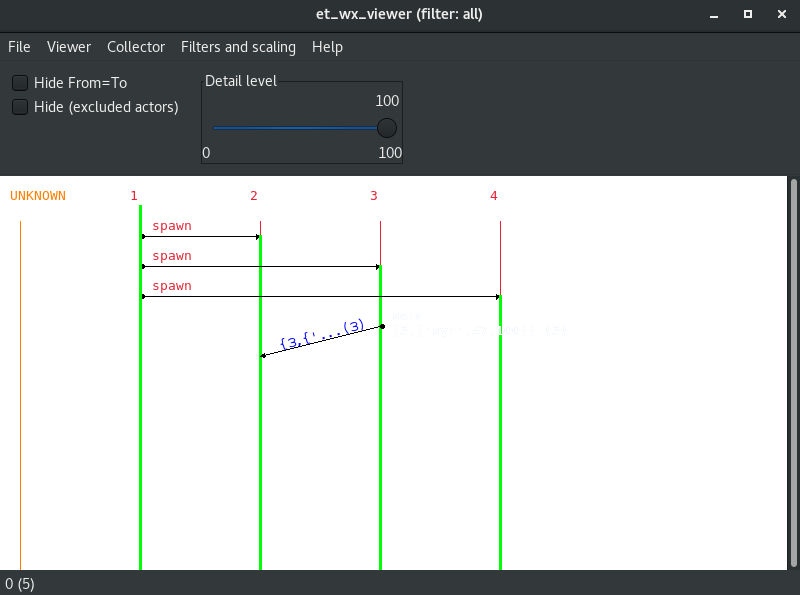
\includegraphics[scale=0.5]{./LavoroLuca/EstensioneCauder/Imgs/GraphicViewerSendReceive}
		\caption{Esempio Graphic Viewer Send/Receive}
		\label{fig6}
	\end{figure}
	Nella figura sottostante mostro un esempio di visualizzazione di uno spaccato dell'esecuzione del seguente codice Erlang, a cui associo le varie regole che spiegherò nella semantica in avanti:
		\lstinputlisting{./LavoroLuca/EstensioneCauder/esempio.erl}
	Il processo 1 setta il suo \textit{process\_flag} a \textit{true} e spawna con link il processo 2. Successivamente il processo 2 spawna con link il processo 3, per poi proseguire con l'intera esecuzione fino alla propria \textit{terminazione del codice}. Alla terminazione, il processo 2 esegue la \textit{propagazione del segnale}. Dopo di chè vengono schedulati i vari segnali propagati. Da notare come il segnale propagato dopo (con time=2) venga schedulato prima del segnale con time=1.
	\begin{figure}[H]
		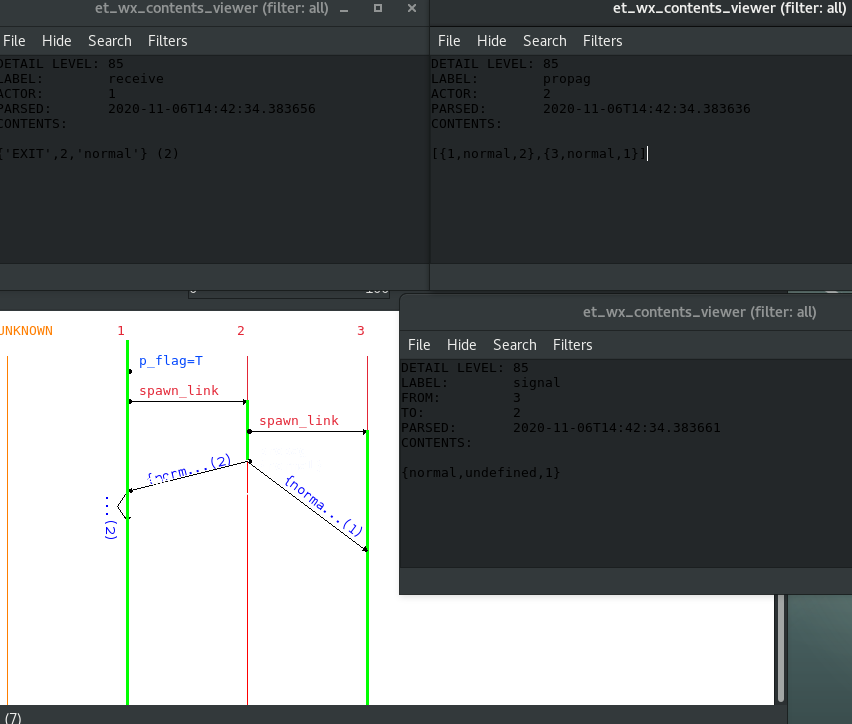
\includegraphics[scale=0.5]{./LavoroLuca/EstensioneCauder/Imgs/GraphicViewerEsteso}
		\caption{Esempio Graphic Viewer Esteso}
		\label{fig7}
	\end{figure}
	\begin{itemize}
		\item $\mathsf{Process\_flag}$: 
		La chiamata a $\mathsf{process\_flag}$, oltre a settare il flag del processo al valore booleano passato come argomento, ritorna il vecchio flag del processo che chiamerò \textit{OldBool}.
		Ciò si concretizza in Cauder, cambiando il campo \textit{f} di P in \textit{f'} settato a \textit{Bool}, mentre \textit{h} di P evolve $\displaystyle h'=[\{\mathsf{process\_flag},\theta,e,OldBool\} \mid h ]$.
		Sia P'=$\displaystyle \langle p,\theta,e',h',lm,l,f'=Bool \rangle$, lo stato risultante da questo passaggio sarà
		S'=$\displaystyle \Gamma;\Psi;\Pi\setminus\{P\}\cup\{P'\}$.\\
		Nel graphic viewer, in relazione alla figura \ref{fig7}, $\mathsf{process\_flag}$ viene mostrata tramite la label \textit{p\_flag=Bool} con Bool= T (true) or F (false).
		\item $\mathsf{Spawn\_link}$: 
		La funzione $\mathsf{spawn\_link}$ è molto simile alla funzione $\mathsf{spawn}$, con la differenza che opera anche sui link tra processi, per cui nella descrizione della semantica di essa, tratterò solo la parte relativa ai link.\\
		La chiamata a $\mathsf{spawn\_link}$, oltre a creare un nuovo processo P' vuoto, setta i relativi link nei due processi coinvolti.\\
		Più formalmente, viene creato un P'=$\displaystyle \langle p',\theta'= \emptyset,e',h'=[],lm'=[],l'=\{p\},f'=false \rangle$, mentre P evolve in P''=$\displaystyle \langle p,\theta,e'',h'',lm,l''=l \cup\{p'\},f \rangle$ \\con h''=$\displaystyle [\{\mathsf{spawn\_link},\theta,e,p'\} \mid h]$.
		Il sistema risultante da questo passaggio sarà S'=$\Gamma$;$\Psi$;$\Pi$$\setminus$\{P\}$\cup$\{P',P''\}.
		Nel graphic viewer, in relazione a \ref{fig7}, $\mathsf{spawn\_link}$ viene mostrata tramite la label \textit{spawn\_link}.
		\item $\mathsf{Error~e~exit}$: 
		Semanticamente, queste due regole sono molto simili tra loro, in quanto aggiungono o tolgono lo stesso tipo di informazioni.Indico con \textit{call}= $\mathsf{error}$ se avviene una chiamata ad $\mathsf{error}$ o $\mathsf{exit}$ se avviene una chiamata ad $\mathsf{exit}$, mentre con \textit{callExp}\footnote{Sarebbe l'espressione risultante dalla chiamata ad una di esse.Da notare che entrambe le chiamate non hanno nessun valore di ritorno, ma gli si associa una delle tuple di seguito per indicare la terminazione e che tipo di terminazione.}
		\{$\mathsf{exit}$,Reason\} nel caso di chiamata ad $\mathsf{exit}$ o \{$\mathsf{error}$,Reason,stack\} nel caso di chiamata ad $\mathsf{error}$.\\
		Sia h'=$\displaystyle [\{call,\theta,e,Reason\} \mid h]$.
		Il processo P evolve in P'=$\displaystyle \langle p,\theta,e'=callExp,h',lm,l,f \rangle$, con il sistema S che evolve in S'=$\displaystyle \Gamma;\Psi;\Pi\setminus\{P\}\cup\{P'\}$.
		Non essendo visualizzato nel tab \textit{trace} di Cauder, non lo rappresento neanche nel graphic viewer.\\
		\item $\mathsf{Propagazione~dei~segnali}$:
		Concettualmente, la propagazione dei segnali risulta essere molto simile alla \textit{rule send}, in quanto un carico di informazioni viene inviato e immagazzinato in una struttura dati aggiuntiva in attesa di essere consegnata.
		Può essere vista come una \textit{send uno-a-tanti}.\\
		Per ogni link di P viene generato un segnale ed inviato al processo linkato, prima che P termini del tutto.\\
		Più formalmente:\\
		Sia histSignals=$\displaystyle \bigcup_{link \in l}\{link,type,reason,time\}$.\\
		Sia h'='=$\displaystyle[\{\mathsf{propag},\theta,e,histSignals\} \mid h]$.\\
		Allora P evolve in P'=$\displaystyle \langle p,\theta,e',h',lm,l'=[],f \rangle$.\\
		Sia signals=$\displaystyle \bigcup_{hist \in histSignals}\{hist.link,p,hist.type,hist.reason,hist.time\}$.\\
		Allora il sistema S evolve in S'=$\displaystyle \Gamma;\Psi \cup signals;\Pi \setminus \{P\} \cup \{P'\} $.\\
		Nel graphic viewer la propagazione dei segnali verrebbe mostrata con la label \textit{propag\{Type,Reason\}} con \textit{Type}=$\mathsf{error}$ o $\mathsf{normal}$ e \textit{Reason}= $\mathsf{undefined}$ se \textit{Type}=$\mathsf{normal}$.\\
		In relazione alla figura \ref{fig7} la propagazione dei segnali viene mostrata tramite l'et\_context\_viewer con \textbf{label}=propag, con le varie informazioni sui segnali inviati.
		\item $\mathsf{Ricezione~segnali}$:
		La trattazione dei segnali è molto simile a quella dei messaggi, seppur vengono coinvolte strutture dati diverse e vengano prodotti effetti diversi.\\
		Il percorso di un segnale è del tipo: $\displaystyle invio\xrightarrow{prop}\Psi\xrightarrow{signal}ricezione$, mentre quello di un messaggio è del tipo: $\displaystyle invio\xrightarrow{send}\Gamma\xrightarrow{sched}lm\xrightarrow{receive}ricezione$.\\
		Concettualmente la ricezione dei segnali ingloba atomicamente al suo interno la \textit{rule sched} e la \textit{rule receive}, ovviamente trattando un carico di informazione diverso e con effetti diversi.
		Come precondizione per effettuare una schedulazione del segnale ad un processo P, bisogna che esso sia vivo, ovvero che \textit{e} sia effettivamente una espressione.\\
		\textit{Questa precondizione si applica a tutte le casistiche che verranno proposte}.
		Posto che vi sia questa condizione, si presentato 4 casistiche relative alla ricezione dei segnali, che dipendono dal valore del \textit{process\_flag} del processo ricevente.\\
		Per ognuna delle casistiche, il sistema  S evolve  togliendo il segnale schedulato da $\Psi$ e aggiungendo P' e togliendo P ad $\Pi$, quindi presenterò solo come evolve P in P', sottintendendo, alla fine, l'evoluzione di S in S'.
		Quindi selezionato il segnale da schedulare, \textbf{in base al time}, se:
			\begin{enumerate}
			\item signal.type=$\mathsf{error}$ $\wedge$ f=$\mathsf{true}$:\\
				Sia lm'=$\displaystyle [\{\{\mathsf{EXIT},signal.from,signal.reason\},signal.time\} \mid lm]$.\\
				Sia h'=$\displaystyle[\{\mathsf{signal},signal.from,error,signal.reason,signal.time\} \mid h]$.\\
				Il processo P evolve in P'=$\displaystyle \langle p,\theta,e,h',lm',l'=l\setminus\{signal.from\},f \rangle$.
			\item signal.type=$\mathsf{error}$ $\wedge$ f=$\mathsf{false}$:\\
				Sia h'=$\displaystyle [\{\mathsf{signal},signal.from,error,\theta,e,signal.time\} \mid h]$.\\
				Il processo P evolve in P'=$\displaystyle \langle p,\theta,e'=\{\mathsf{error},signal.reason,stack\},h',lm,l'=l \setminus\{signal.from\},f \rangle$.
				Il motivo per cui viene tolto solo il link del processo che ha inviato il segnale, risiede nel fatto che il processo ricevente potrà ripropagare a tutti i suoi processi linkati il segnale di errore appena ricevuto.
			\item signal.type=$\mathsf{normal}$ $\wedge$ f=$\mathsf{true}$:
				Il processo P evolve in P' in maniera simile al caso 1, con l'unica differenza nel campo h', che viene aggiunta la tupla \{'signal',signal.from,normal,signal.time\} al posto dell'altra, che segnala un terminazione normale del codice.
			\item signal.type=$\mathsf{normal}$ $\wedge$ f=$\mathsf{false}$:
				Il processo P evolve in P' in maniera simile al caso 3, con l'unica differenza che non viene creato il messaggio, ma viene solo rotto il link col processo che ha propagato il segnale.
			\end{enumerate}
		In relazione alla figura \ref{fig7}, l'et\_context\_viewer con \textbf{label}= signal) mostra la ricezione del segnale con time=1 da parte del processo 3.\\
		Il processo 1 avendo il \textit{process\_flag} a \textit{true}, dopo la ricezione del segnale con time=2 (\textbf{il punto di partenza della freccia spezzata}, avrebbe l'et\_context\_viewer simile a quello con label=signal), converte in messaggio il segnale ricevuto, e ne effettua la \textit{receive}, com mostrato nel et\_context\_viewer con \textbf{label}= receive.
	\end{itemize}
\textbf{SEMANTICA ALL'INDIETRO}:
	\begin{itemize}
		\item $\mathsf{Process\_flag}$: Avendo h=$\displaystyle [\{\mathsf{process\_flag},\theta_{old},e_{old},OldBool\} \mid h']$, per effettuare l'undo del process flag, banalmente si crea un P'= $\displaystyle \langle p,\theta_{old},e_{old},h',lm,l,f'=OldBool \rangle$.\\
		Il sistema evolve come nella semantica in avanti, togliendo P ed inserendo P'.
		\item $\mathsf{Spawn\_link}$:
		Per poter effettuare un passo all'indietro della spawn\_link, si ha la stessa precondizione relativa alla spawn, ovvero il processo spawnato deve essere "vuoto". \\
		Avendo h=$\displaystyle [\{\mathsf{spawn\_link},\theta_{old},e_{old},p_{spawn}\} \mid h']$,\\
		si crea un processo P''=$\displaystyle \langle p,\theta_{old},e_{old},h',l'=l \setminus \{p_{spawn}\},f \rangle$.
		Il sistema evolve in S'=$\displaystyle \Gamma;\Psi;\Pi\setminus\{P,P'\}\cup\{P''\}$.
		\item $\mathsf{Error~e~exit}$: Sia h=$\displaystyle [\{call,\theta_{old},e_{old},Reason\} \mid h']$.\\
		Banalmente, il processo P evolve in P'=$\displaystyle \langle p,\theta_{old},e_{old},h',lm,l,f \rangle$ ed S evolve allo stesso modo della semantica in avanti.
		\item $\mathsf{Propagazione~dei~segnali}$: Per effettuare l'undo di una propagazione dei segnali, bisogna che tutti i segnali inviato dal processo morente siano presenti in $\Psi$.
		Se non si rispettasse questa condizione, quindi si potesse fare l'undo in ogni momento della propagazione, si rischierebbe di violare la consistenza causale.\\
		Ipotizziamo di avere $\Psi$=[\{1,2,error,badarg,1\},\{3,2,error,badarg,2\}], a seguito di una propagazione da parte del processo 2. Ora se schedulassi in avanti il segnale di tempo=1 avrei $\Psi$=[\{3,2,error,badarg,2\}], ma cosa ben più importante, essa ha prodotto degli effetti sul processo che lo riceve(più avanti si vedrà la regola della consegna dei segnali). Se ora annullassi la propagazione senza aver annullato prima la schedulazione del segnale, otterrei che il processo 1 ha subito degli effetti da parte della schedulazione di un segnale che non è mai esistito.
		Posta che vi sia questa condizione, l'undo della propagazione ritira tutti i segnali emessi dal processo morente, ricreando i link rotti.
		Più formalmente:\\
		Sia h=$\displaystyle [\{\mathsf{propag},\theta_{old},e_{old},histSignals\} \mid h']$.\\
		Sia oldLinks=$\displaystyle  \bigcup_{histSig \in histSignals}histSig.link $.\\ 
		Sia signals=$\displaystyle \bigcup_{histSig \in histSignals}\{histSig.link,p,histSig.type,histSig.reason,histSig.time\}$.\\
		Allora P'=$\displaystyle \langle p,\theta_{old},e_{old},h',lm,l=oldLinks,f \rangle$.
		Il sistema S evolve in S'=$\displaystyle \Gamma;\Psi \setminus signals;\Pi \setminus \{P\} \cup \{P'\} $.
		\item \underline{Ricezione segnali}: Anche nell'undo della schedulazione di un segnale si presentato 4 casistiche, in funzione delle informazioni in \textit{h} ed eventualmente di \textit{f} in quell'istante.
		Ogni casistica può avere una sua precondizione, che definisco in quella specifica casistica.
		In ogni casistica, dopo aver evoluto P in P', ciò che viene fatto è:
		\begin{enumerate}
			\item Ricreare il segnale \textit{signal}, date le informazioni necessarie nella history, ed evolvere $\Psi$ in $\Psi'$=$\Psi$ $\cup$ \{signal\}.
			\item Evolvere $\Pi$ in $\Pi'$=$\Pi$ $\setminus{P}$ $\cup{P'}$.
			\item Evolvere il sistema S in S'=$\displaystyle \Gamma;\Psi';\Pi'$.
		\end{enumerate}
		Qui di seguito espongo la regola dell'undo di un segnale,secondo le varie casistiche, illustrando solo come evolve P in P':
		\begin{enumerate}
		\item h=$\displaystyle [\{\mathsf{signal},from,\mathsf{error},reason,time\} \mid h']$:\\
			  Indica un ricezione di un  segnale di errore $\wedge$ \textit{f}=$\mathsf{true}$(vedi h del caso 1 nella semantica in avanti).
			  Come precondizione, questa casistica necessita che il relativo messaggio derivato dal segnale, \textit{sia in cima ad lm}, ovvero lm=$\displaystyle [\{\{\mathsf{EXIT},signal.from,signal.reason\},signal.time\} \mid lm']$. Se non ci fosse questa precondizione, si rischierebbe di violare il Loop Lemma. Ipotizziamo di essere in questa situazione:
			  lm=[\{\{$\mathsf{EXIT}$,error,reason\},2\},\{"ciao",3\}].Se facessi l'undo del segnale, per poi rischedularlo al passo successivo, mi troverei con lm=[\{"ciao",3\},\{\{$\mathsf{EXIT}$,error,reason\},2\}], ovvero il messaggio generato dal segnale si ritroverebbe in testa.
			  Da uno stato S, ho fatto l'undo di un'azione per poi rifarla e mi son ritrovato in uno stato S'$\neq$S, infrangendo il Loop Lemma.
			  Detto questo, avendo lm=$\displaystyle [\{\{\mathsf{EXIT},signal.from,signal.reason\},signal.time\} \mid lm']$, \\si ha P'=$\displaystyle \langle p,\theta,e,h',lm',l \cup \{from\},f \rangle$.
			  Da notare che $\theta$ ed \textit{e} rimangono inalterati.
		\item h=$\displaystyle [\{\mathsf{signal},from,\mathsf{error},\theta_{old},e_{old},time\} \mid h']$:\\
			  Indica una ricezione di un segnale di errore $\wedge$ \textit{f}=$\mathsf{false}$(vedi h del caso 2 nella semantica in avanti).
			  Per la ricostruzione del segnale \textit{signal}, \textit{reason} la posso tranquillamente ricavare dal secondo elemento di \textit{e}.
			  Detto ciò, evolvo P in P'=$\displaystyle \langle p,\theta_{old},e_{old},lm,l \cup \{from\},f \rangle$.
		\item h=$\displaystyle [\{\mathsf{signal},signal.from,\mathsf{normal},signal.time\} \mid h']$:\\
			  Indica una ricezione di terminazione normale.
			  In questo caso il tipo di comportamento della regola, lo posso discriminare in base a \textit{f} in quell'istante.
			  \textit{Sia f}=$\mathsf{true}$.\\
			  Allora diventa analogo al caso 1 della semantica all'indietro, ovviamente ricostruendo un \textit{signal} di type=$\mathsf{normal}$.
			  \textit{Sia f}=$\mathsf{false}$.\\
			  Banalmente P evolve in P'=$\displaystyle \langle p,\theta,e,h',lm,l \cup \{from\},f \rangle$.
	\end{enumerate}
	\end{itemize}
\textbf{ROLLBACK}:\\
	Risultano essere interessanti solo due regole ai fini dell'operatore \textit{roll}, in quanto sono gli unici che risultano avere conseguenze che si ripercuotono su altri processi.
	A dire il vero ne esiste una terza (roll\_signal) ma, come si vedrà a breve, essa viene inglobata nella \textit{roll della propagazione dei segnali}.
	\begin{itemize}
		\item \underline{Propagazione segnali}:\\
		Sia h=$\displaystyle [\{\mathsf{propag},\theta,e,histSignals\} \mid h']$.
		Bisogna creare la condizione per cui si possa ripropagare all'indietro.
		Algoritmicamente, la roll di un propagazione si sviluppa in questo modo:\\
		\begin{algorithm}[H]
		\caption{roll\_propag(State,Pid)}
		\begin{algorithmic}
		\FORALL {histSignal $\in$ histSignals} 
			\STATE Signal=recreateSignal(histSignal,Pid)
			\STATE State=roll\_signal(State,Signal)
		\ENDFOR
		\RETURN back\_propag\_step(State,Pid)
		\end{algorithmic}
		\end{algorithm}
		La funzione \textit{recreateSignal} si occupare di ricreare il \textit{record signal} con le informazioni che gli vengono passate. 
		A livello molto generico ed informale, la \textit{roll\_signal} va a creare la condizione per cui il segnale possa essere ritirato.
		Più in dettaglio, se il segnale può essere ritirato direttamente allora termina, altrimenti fai fare un passo indietro \textit{al processo che lo ha ricevuto} e rivaluta \textit{roll\_signal} sul segnale ricorsivamente, finchè non si arriva al caso base.
		In termini algoritmici, la roll\_signal si sviluppa in questo modo:\\
		\begin{algorithm}[H]
		\caption{roll\_signal(State,Signal)}
		\begin{algorithmic}
		\IF {Signal $\in$ $\Psi$} 
			\RETURN State
		\ELSE
			\STATE DestPid=Signal.p'
			\STATE State'=back\_step(State,DestPid)
			\RETURN roll\_signal(State',Signal)
		\ENDIF
		\end{algorithmic}
		\end{algorithm}
		\item \underline{Spawn\_link}:\\
			La roll della spawn\_link risulta essere identica alla roll della spawn.
			Ovvero viene creata la condizione per cui una spawn possa essere invertita, cioè si annullano \textbf{tutte} le azione effettuate dal processo spawnato, per poi invertirla,
			secondo la regola all'indietro della spawn\_link.
	\end{itemize}
\subsection{Un esempio di Cauder esteso}
Il codice che mostro qui sotto implementa una comunicazione client-server e viene mostrato in figura \ref{example}.\\
Un \textit{server} riceve delle richieste da 2 \textit{client}.\\
Il server inoltre mantiene una memoria in cui mappa i worker con i relativi client.\\
Questi 2 \textit{client} inviano ognuno 2 valori presi da una lista predefinita di valori per ottenere in output dal \textit{server} una divisione.\\
Finchè non riesce a soddisfare una richiesta, il \textit{client} continua ad inviare richieste, scegliendo ogni volta degli input casuali dalla lista di valori.\\
In questa lista sono presenti dei valori non numerici per simulare una richiesta malformata che il \textit{server} deve gestire.\\
Ad ogni richiesta ricevuta il \textit{server} spawna un \textit{worker} che esegue effettivamente la divisione e che si occupa di inviarla al rispettivo \textit{client}.
Nel caso il \textit{worker} non riuscisse a gestire la richiesta, il server dovrebbe occuparsi di riferire al client l'errore, mentre nel caso riuscisse a gestirla e quindi terminare correttamente, il server provvede a rimuoverlo dalla memoria.
La procedura di debugging si articolerebbe nei seguenti passi, utilizzando la modalità \textit{manual} e facendo riferimento a \ref{dbg}:
\begin{enumerate}
	\item Avviare il \textbf{server} (Proc. 2 in figura) e metterlo in ricezione eseguendo un passo con esso.
	\item Avviare un \textbf{client} (Proc. 3 in figura) ed eseguire dei passi finchè non arriva alla \textit{send} di un messaggio verso il server.
	\item Quando il \textit{msg} viene inserito nella \textit{GM} porre attenzione al \textit{payload}.
	\item \underline{Schedulare} il \textit{msg} al \textbf{server}, tramite il \textit{time} di \textit{msg}.
	\item A questo punto proseguire col server, ricevendo il \textit{msg} e avviare un \textbf{worker}.
	\item Ora è il momento di far lavorare il \textbf{worker} eseguendolo fino alla fine. A questo punto ci sono due casistiche:
		\begin{itemize}
			\item Il \textbf{worker} riesce a fare la divisione e quindi invia al \textbf{client} il risultato ed esce. A questo punto è pronto per la \textit{propagazione dell'uscita} al server, che eseguo. Nella \textit{GS} compare il \textit{signal} di tipo $\mathsf{normal}$ che schedulo tramite il suo \textit{time} schiacciando il pulsante \textit{Signal} nella modalità \textit{Manual}. Ora, guardando sullo stato di Proc. 2, dovrebbe essere visualizzata in \textit{H} la ricezione del \textit{signal} col relativo messaggio in \textit{LM}, pronto per essere estratto ed elaborato, per poter rimuovere il \textbf{worker} della memoria del server.
			In tal caso o avviare un'altro \textbf{client} oppure usare l'operatore \textit{roll} nella modalità \textit{Rollback} per fare l'undo della \textit{spawn} del \textbf{client} e ripetere il procedimento, tentando di andare in errore.
			\item Il worker non riesce a fare la divisione. A questo punto essendo andato in errore è pronto per la \textit{propagazione dell'errore} al server, che eseguo. Schedulo il segnale di errore in maniera analoga al punto precedente. Ora, guardando sullo stato di Proc. 2, dovrebbe essere visualizzata in \textit{H} la ricezione del \textit{signal} col relativo messaggio in \textit{LM}, pronto per essere estratto ed elaborato, per poter avvisare il \textbf{client} dell'errore della richiesta.
		\end{itemize}
\end{enumerate}
\begin{figure}[!ht]
\lstinputlisting{./LavoroLuca/EstensioneCauder/EsempioDebug/clientServer.erl}
\caption{client-server}
\label{example}
\end{figure}
\begin{figure}[!ht]
\centerline{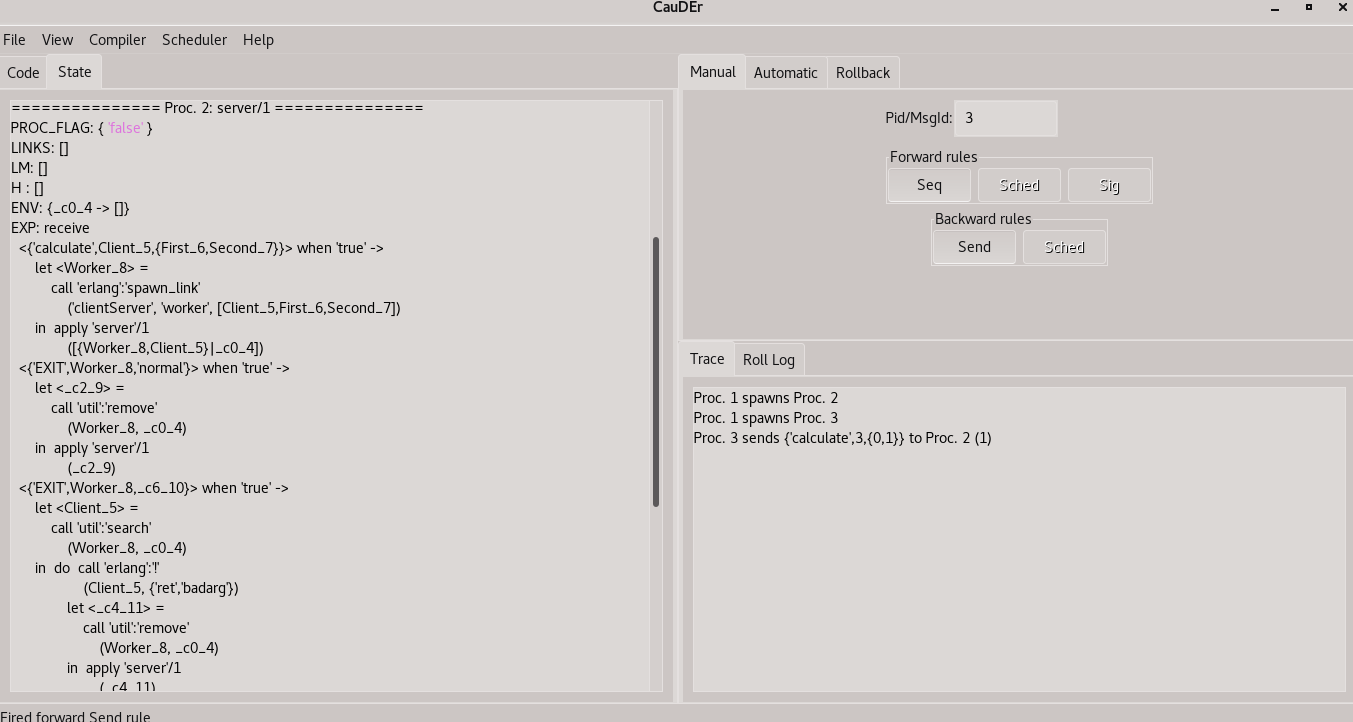
\includegraphics[scale=0.4]{./LavoroLuca/EstensioneCauder/EsempioDebug/ScreenDebug}}
\caption{client-server Cauder}
\label{dbg}
\end{figure}
Il video può essere trovato al link \href{https://github.com/Taba92/Tesi}{https://github.com/Taba92/Tesi} con il nome del file \textit{luca.mkv}.
\end{document}